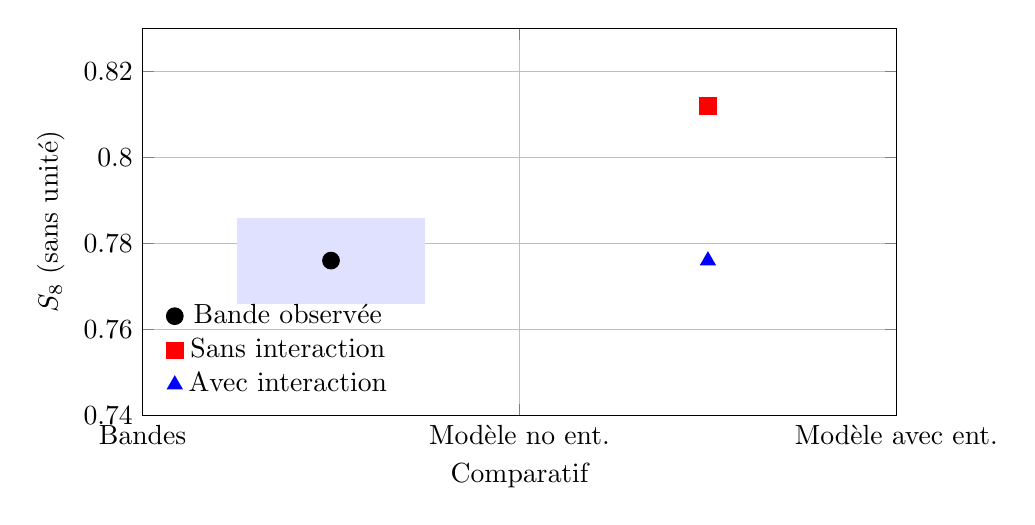
\begin{tikzpicture}
\begin{axis}[
    width=0.92\linewidth,
    height=6.5cm,
    xlabel={Comparatif},
    ylabel={$S_8$ (sans unité)},
    xmin=0, xmax=2,
    ymin=0.74, ymax=0.83,
    xtick={0,1,2},
    xticklabels={Bandes,Modèle no ent.,Modèle avec ent.},
    grid=both,
    legend style={at={(0.02,0.02)},anchor=south west,draw=none,fill=none},
]
\path[fill=blue!12] (axis cs:0.25,0.766) rectangle (axis cs:0.75,0.786);
\addplot[only marks,mark=*,mark size=3pt,black] coordinates {(0.5,0.776)};
\addlegendentry{Bande observée}
\addplot[only marks,mark=square*,mark size=3pt,red] coordinates {(1.5,0.812)};
\addlegendentry{Sans interaction}
\addplot[only marks,mark=triangle*,mark size=3pt,blue] coordinates {(1.5,0.776)};
\addlegendentry{Avec interaction}
\end{axis}
\end{tikzpicture}